\documentclass{report}

% Allows you to insert special characters (UTF8)
\usepackage[utf8]{inputenc}

% Language used in the document.
\usepackage[UKenglish]{babel}


% -- Pictures
% Allows to insert pictures
\usepackage{graphicx}

% Allows to force positioning of pictures
\usepackage{float}

% Load eps files (MATLAB files)
\usepackage{epstopdf}


% -- Mathemtatics
% Additional mathematics
\usepackage{amsmath}

% Shortcuts for many physics related things.
% CAUTION: YOU MUST HAVE MCODE.STY FILE IN YOUR PROJECT
\usepackage{physics}

% Display measurement data easily
\usepackage{siunitx}
\sisetup{separate-uncertainty=true, multi-part-units=single, exponent-product=\cdot}

% -- Layout
% Change page size to use more normal margins
\usepackage{fullpage}

% Change how paragraphs are formatted
\usepackage{parskip}

% Allows you to make two of three column documents (e.g. papers)
\usepackage{multicol}

% Insert URLs
\usepackage[hidelinks]{hyperref}


% -- Organisation
% Allows you to use subfiles (very useful!)
\usepackage{subfiles}


% -- References
% Use the bibLaTeX package.
% CAUTION: YOU MUST ADDITIONALLY TELL LATEX WHICH LIBRARY YOU ARE USING WITH:
%          \addbibresource{main.bib}
%
%          Afterwards you can create the bibliography using
%          \printbibliography[heading=bibintoc,title={References}]
%          (The bibintoc adds the references to the table of contents)
\usepackage[style=numeric]{biblatex}

\graphicspath{ {./images/} }
\addbibresource{tetris.bib}
\usepackage{todonotes}
\title{Learning to play Tetris using deep Q learning}
\author{Coen Verschuur \and Emiel Slootman}
\date{\today}

\begin{document}

\maketitle


\section{Introduction}
Tetris. Who doesn't know it. Tetris was developed in the 80's by the Sovjet engineer Alexey Pajitnov at the Moscow Academy of Science \cite{tet}. The point of the game is to drop blocks, tetrominos, and make full rows which gets you point. To be successful at the game insight and a certain speed are required of the player. You have to be tactical about how you drop the blocks and how you orientate them. If you just roughly keep dropping the blocks in the places were there are big holes, you are gonna find you are quickly developing holes. Besides, it is worth it to wait out on clearing a line if this allows you to clear multiple lines are once in a later turn, since this yields a higher score. This last fact makes Tetris a very suitable game for a reinforcement learning approach.
In this report we will first go over some basic theory about reinforcement learning. After this we will talk in more detail about how to approach Tetris using reinforcement learning and then we will discuss how we implemented a reinforcement learning algorithm to play Tetris.

\subsection*{Source}
You can find all our source code and the results from all the experiments we did in our github repository which can be found at \url{github.com/Mielleman201/ML-Tetris}. Here all our python files are present. All our measurement results can be found in the folder 'data'.

\tableofcontents

\chapter{Theory}
\section{Reinforcement Learning \label{sec:RL}}
In reinforcement learning, the learner has to learn which actions to take in order to maximise a reward \cite[1]{Sutton2018}. The learner does not know what he is looking at or what his actions do. Reinforcement learning is focused on studying the behaviour of such agents, the object that is learning, and how they behave and how they can be optimised. A famous example of a reinforcement learning algorithm is AlphaGo \cite{alphago}. AlphaGo was the first computer program that was able to beat the world champion in Go. Go in an ancient Chinese board game which is famous for it's complexity. AlphaGo makes use of neural networks, like most reinforcement learning algorithms, to predict which moves are the best.

% Reinforcement learning is different from supervised learning. In supervised learning, the training data is already labelled with the correct output \cite[2]{Sutton2018}. The goal of the algorithm is to give the correct response for new data which are not in the training data, for playing a game this means that it will never be better than the input. In reinforcement learning there is no pre-labelled data. The agent must explore on its own and learn from its own experience. An important part of this learning is the Markov decision process.

The difference between reinforcement learning and other types of learning paradigms, is that reinforcement learning doesn't make use of a pre-defined learning data set \cite[2]{Sutton2018}, the data set is not independent and identically distributed. This means that it has to learn on its own, and that is done with a reward. The reward is very important, that makes it at the same time also hard to do right. In most of the cases the reward is based on the complete series of actions that are taken to come to the end result. This means that the reward is given to a series of actions, and which of the actions resulted in the good end result, that is the question.

\subsection{The reward}
The reward is a variable that scales the feedback signal, and that gives the agent feedback on its actions. The agent scores points for actions that are favourable, and can also loses points for actions that have a bad effect on the end result. Reinforcement learning is based on the Reward Hypothesis which states that, "All goals can be described by the maximisation of expected cumulative rewards."\cite{RL_intro}.

For example, we want to learn a person to walk. We can break down his actions necessary to walk. We can give points for the displacement in the right direction, but at the same time we can give him penalties for every time it falls. The agent wants to optimise its reward. After some time have learnt that some actions are good and some actions are bad, and that it will stimulate the good actions. This would hopefully result in an agent that would not fall over and would hopefully be able to take some steps.

\begin{figure}
    \centering
    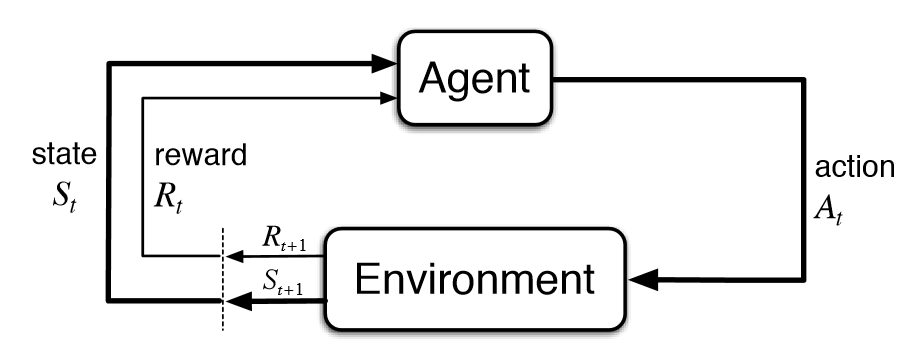
\includegraphics[width=0.75\textwidth]{verslag/images/reinforcement_learning_diagram.png}
    \caption{A schematic representation of how reinforcement learning works.\cite{RLimg}}
    \label{fig:reinforcement_diagram}
\end{figure}

\subsection{Agent and environment}
In figure (\ref{fig:reinforcement_diagram}) you can see a simple diagram of the interaction between the agent and the environment. The environment gives a new state and a reward for a action that the agent took, after that the agent will decide a new action based on the state and reward. Every loop of interaction between agent and environment is called a time step, and every variable is stored in the history. The history is what the agent has seen for so far.  The agent can determine his actions based on the history. This looks like a great option to map the current state on the states you have seen before, but the history is not very useful since it’s enormous, and it’ll be infeasible to use this approach in the real-world interesting problems.

\subsection{Agent and environment state}
The environment state is the information used within the environment to determine what has to happen next viewed form the environment’s perspective. The environment state is a private representation of the environment to pick the next state and reward. In general, the environment’s state is not visible for the agent, and if it is visible for the agent, it might contain some irrelevant information. The agent has its own state, that captures what happened to the agent so far. The agent makes a choice based on that state, it is like a summery of what is going on. The agent state can be any function of the history, and this state is made by the agent himself.

An information state also called a Markov state contains all useful information form the history. The Markov state is used to represent the agent’s state. "A state St is Markov if and only if; $P[St +1\mid St] = P[St+1 \mid S1,...,St]$"\cite{RL_intro}.

This results in that the agent state is Markov if that state contains all the useful information for the agent. Which results in that we can throw away all the previous states, since they are already represented by the agent’s current state. This resulted in the well known quote: “The future is independent of the past given the present.”. The Markov Decision processes will be further explained in section \ref{sec:MDP}.

There are a lot of different kind of agents, we will only discus the components that can be combined to create our agent. In a later stage we will explain our choice. The first component is a policy, this could be a deterministic policy, that we want to learn from experience,
\begin{align}
    a=\pi(s)    
\end{align}
or a stochastic policy,
\begin{align}
    \pi(a|s)=p[A_t=a|s_t=s]
\end{align}
The second component is a Value Function, this gives a prediction for the expected future reward, this makes it possible to decide if it better to get the points now or later on.
And third and last, a Model, a model will predict what the environment will do next. It’s the agent’s representation of the environment, How the agent thinks the environment works.

\section{Finite Markov decision process \label{sec:MDP}}
The Markov decision process is like an algorithm for the computer to take a decision. This decision is a policy, and is build out of changes. The agent wants to maximise its reward, so the policy will take actions that will result in the highest reward. But it is not always the best choice to take the reward in the short run, sometimes it is better to wait, and take the points later on. And this is what the Markov decision process is about, to make the right choices at the right moment, and maximise your reward.

The Markov decision process uses the variables that are already described in section \ref{sec:RL}:\newline
States: S\newline
Model: T(S,A,S') $\rightarrow$ Pr(S' $\mid$ S,A)\newline
Actions: A(S), A\newline
Reward: R(S), R(S,A), R(S,A,S')\newline
Policy: $\pi(S) \rightarrow A$ and/or $\pi^*$\newline

So, the state (S) is the current state the environment is in and S' is the next state. But the state doesn't have to describe only the current state, it can also describe the state in which the environment has been. Which will go back to the Markov principle: "The future is independent of the past given the present." and that can be very helpful since we have one variable instead of the complete history. Next we have the actions (A) this are simply the actions the agent can do in a particular state. Then we have the model, which describes the rules for the environment. It is like the physics for the environment. It uses the current state and the next state, with the action needed to go to that next state, and it will give return the probability that the environment will get in that next state. So, the sum of all probabilities of the actions will be one, since we need to take an action in a next step. The model is constant and won't change during the complete process. What isn't constant is the reward that is given for a certain action. There are three definitions given for the reward, but in the mathematical world they are the same, it is always possible to put some history in to the current state, this is a property of the Markov decision process.

\subsection{Policies and value functions}
We have just describe the problem, but of course you also want a solution for this problem, and that is the policy ($\pi(S)$). The policy is a function that takes a state, and returns an action. But besides the policy $\pi$ we also have a long term policy ($\pi^*$) and this will maximise your long term expected reward. So, the amount of points you will have in the end of the live time.

The policy is also one the biggest differences between reinforcement learning and other types of learning paradigms. The difference is that by reinforcement learning there are more options to make an action. For supervised learning, we have a certain state, and we know which action is associated with that state. In reinforcement learning we have a certain state, and we have a few action we can do, but every action gives its own reward. The trick is to optimise the policy.

\section{Evolutionary algorithms}
The evolutionary algorithms that are used now a days are inspired by the evolution theory by Charles Darwin\cite{RL_EA}, The Origin of Species. The working of a machine learning evolutionary algorithms will be explained using the evolution theory by Charles Darwin.

\subsection{Natural selection}
Natural selection is also known as survival of the fittest. This means that the one that has the best genes for its environment has the greatest chance to survive. Which means that the best genes will stay present and the other will slowly disappear. This makes that the species will become as good as the best species that is present in the starting population. In reality the population will keep evolving and become better as a population, but that is related to the reproduction, crossover and mutation.

\subsection{Reproduction and crossover}
A population dies if no new children are born. In the real world, this means that we have to produce children to stay alive. In the process to get new children we crossover some genes, halve of the genes of the man and the women are combined to get a new combination of genes. If the new combinations of genes are successful, the genes will propagate to the next generation of children. In the algorithms we will do the same, we will combine some of the genes to get a new combination, and make it possible to improve the fitness of the species. This will be done by taking the top few percent of the population and combine the genes of those group to make them even better.

\subsection{Mutation}
As genes are copied and relayed from one generation to the next, it can be that during this process mistakes are made. The mistakes are often called mutations. While it are mistakes, it can be very helpful for a population to have them. The mistakes can be bad, and that can result in death, but a mistake can also improve the population and than the mistake can by reproduction continues on in next generations. The reason to want mutations in your population is that not all possible genes are present in the beginning of the population, if you do not have any mutation that means that the end result of the population will highly depend on the starting population.

\section{History of Tetris}
Tetris is at first sight a pretty easy to play game, almost every one has played it before, but behind the scenes it is harder than you would think. All kind of researchers are working for already more than 25 years to make a computer that plays the game better than a Tetris expert, but that has still not happened. We will briefly explain some of the things that are tried before, and what are the results that are obtained with those attempts\cite{Tetris_ML}, We will only have a look at the two methods we have discussed before, so reinforcement and Evolutionary algorithms.

Tetris has a few difficulties that make it hard to use machine learning to play the game, and to compare the results with other people. First, the implementation is different for every person, this means that everyone makes the game slightly different. To give an example, some people will give a point for every line you clear, but others will give you more points if you clear more lines at ones. This is one of the few differences that can be made in the implementation of the game. Second, it happens that the results of the game for change a lot with the same model, because it is a stochastic process. So, to have a good reliable result, we have to play the game a lot of times, but this will take a fair amount of time. A solution for the long play times is that we make the Tetris board smaller, but of course this will have a big effect on the end score.

\subsection{Early attempts}
First we will discuss some early attempts, some of them are really promising, but some of them are almost even worst than a random machine. The results will be given in table (\ref{tab:EA})

\begin{table}[h!]
    \centering
    \caption{The results of some of the earlier attempts for using machine learning for Tetris.}
    \label{tab:EA}
    \begin{tabular}{c|p{4cm}|c|c|p{6cm}}
        Nr. & Name & Year & Result (lines) & Features \\ \hline
        1 & Tsitsiklis \& Van Roy & 1996 & 30 & \begin{itemize}
            \item The number of holes
            \item The height of the highest column
        \end{itemize}\\ \hline
        2 & Bertsekas \& Tsitsiklis & 1996 & 2800 & \begin{itemize}
            \item The height of each column
            \item The difference in height between consecutive columns
        \end{itemize} \\ \hline
        3 & Lagoudakis et al. & 2002 & 1000-3000 & \begin{itemize}
            \item The mean column height
            \item The sum of the differences in consecutive column heights
        \end{itemize} \\ \hline
        4 & Kakade & 2002 & 6800 & \begin{itemize}
            \item Same features as Bertsekas \& Tsitsiklis
        \end{itemize} \\ \hline
        5 & Farias \& Van Roy & 2006 & 4500 & \begin{itemize}
            \item Same features as Bertsekas \& Tsitsiklis
        \end{itemize} \\ \hline
        6 & Ramon \& Driessens & 2004 & 50 & \begin{itemize}
            \item Using patterns of small parts of the grid
        \end{itemize} \\ \hline
    \end{tabular}
\end{table}

For the first two researches in table (\ref{tab:EA}) it was not clear which algorithm they used to get there result, but for the others it was clear. The third research was based on a least-squares policy iteration, the fourth is based on a policy-gradient algorithm, the fifth used a algorithm that samples constraints in the form of Bellman equations for a linear programming solver. For us the most important one is the sixth research, and they used a form of reinforcement learning, but unfortunately they didn't score that good. This was also noticed by Fahey, he decided to hand-craft an agent, so he tuned all the weights by hand. the features he used were:
\begin{itemize}
    \item number of holes
    \item landing height of the piece
    \item number of row transitions
    \item number of column transitions
    \item cumulative number of wells
    \item eroded cells
\end{itemize}

And he did this with a really good result, he made it possible to clear 660.000 lines on average. This is almost a hundred times better than the best result until now. This made clear that it is good possible to use a computer to play Tetris, but so far the best algorithm is not found to get the best result without tuning it by hand.

\subsection{Evolutionary learning}
After the good results of Fahey, other people tried to beat his score of 660.000 and the most promising results came form the evolutionary algorithms. The first result was from B\"ohm et al. (2005) besides the evolutionary algorithms they used, another big change as that they not only used the current Tetrimino, but also the next to come. This resulted in a score of 480.000.000 cleared lines, and is much better than the scores obtained by Fahey.

Szita \& L\"orincz (2006) used the cross-entropy algorithm, the algorithm probes random parameter vectors in search of the linear policy that maximises the score. They achieved a score of 350.000 lines cleared. A year later they also successfully used the cross-entropy algorithm on Ms. Pac-Man.

Thiery \& Scherrer (2009) used the same algorithm, but added a few features. The hole depth and the rows with holes. they achieved a score of 35.000.000 cleared lines. In that same year Boumaza introduced another evolutionary algorithm. The co variance matrix adaptation evolution strategy, his result where very close to the of Dellacherie's, and that is also clear form the amount of lines clear, because also he scored a score of 35.000.000 lines cleared.

So the genetic algorithms gave very good result, much better than all the other algorithms that are tried. The one the came the closest was the hand crafted agent. This changes in 2013 when Gabillon et al. made a reinforcement algorithm based on a classification-based policy iteration algorithm inspired by Lagoudakis \& Parr (2003).

\subsection{Reinforcement learning}
In 2013 Gabillon et al. used a classification-based policy iteration algorithm inspired by lagoudakis \& parr (2003). This algorithm is the first reinforcement algorithm that preforms comparable to the genetic algorithms. What they changed in the algorithm is that they used the sophisticated classifiers inside the loop of reinforcement learning algorithms to identify good actions. Furthermore, they also used estimated values of state-actions pairs with rollouts. The functions of those rollouts where minimized with the CMA-ES algorithm of (Hansen \& Ostermeier, 2001). This is an algorithm that is widely used in the evolutionary algorithms. So, this is a combination of a reinforcement en evolutionary algorithm, this makes that they can make good choices on which actions are good and bad. This makes that the algorithm works much better than the other reinforcement algorithms we have seen so far.


\chapter{Implementation and results}
\section{Short overview of the game}
In this section we will give a short overview of the rules of the game we chose.\\
The board consist of a 8 x 16 matrix. For every block placed, the player receives a point. For every line cleared (so a full lines), the player receives $lines cleared^2 \cdot board width$. So because the board is 8 tiles wide, if the player clears a line using a block, it gets eight points (+1 for placing the block). But if the player clears two lines using one block, the player gets $4\cdot8 = 32$ points for clearing the lines. Additionally, if the tower reaches the top and the player is game over, it losses two points. The game can go on forever, since you can just keep clearing lines to make space. That is why we have determined that we want to reach a goal of 20000 points. We think that an agent who can reach this score is pretty good and going on to higher scores would just take too much time.
Additionally, we have decided that we do not let the agent control the block. For humans, Tetris can also be seen as a game of speed, since you need to make all the right moves in a very short amount of time. For the computer this would be no problem since it can make many orders of magnitude more moves in a second than a human. It would also introduce another layer of complexity to have the agent make moves in real time. That is why we decided we will just feed the neural network all the possible places the block can end up in. This is very limited, because a block can only have a maximum of four rotations and the board is only eight tiles wide, so there never can be more than 32 possible states (usually it is way less since not all blocks have four rotations, and usually there are only six x-coordinates which it can land because of the width of the blocks themselves). You can see two images of the game in figure (\ref{fig:1}) and (\ref{fig:2})
\begin{figure}[h!]
	\centering
	\begin{minipage}[t]{0.45\textwidth}
   		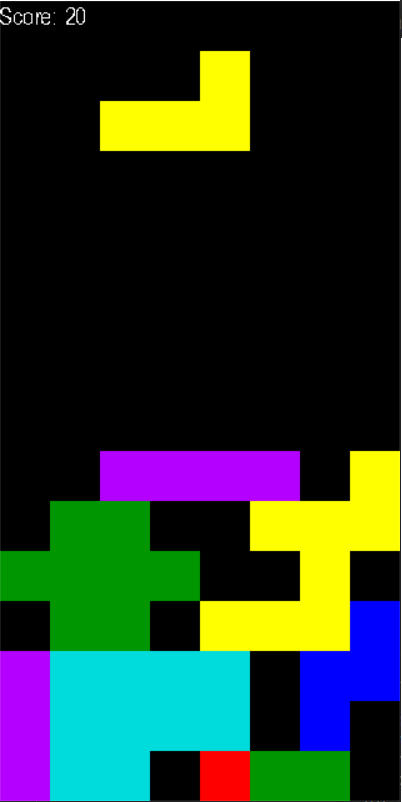
\includegraphics[width=\textwidth]{/tetrisexample1.png}
    	\caption{Example of the game}
    	\label{fig:1}
 	\end{minipage}
  	\begin{minipage}[t]{0.45\textwidth}
    	 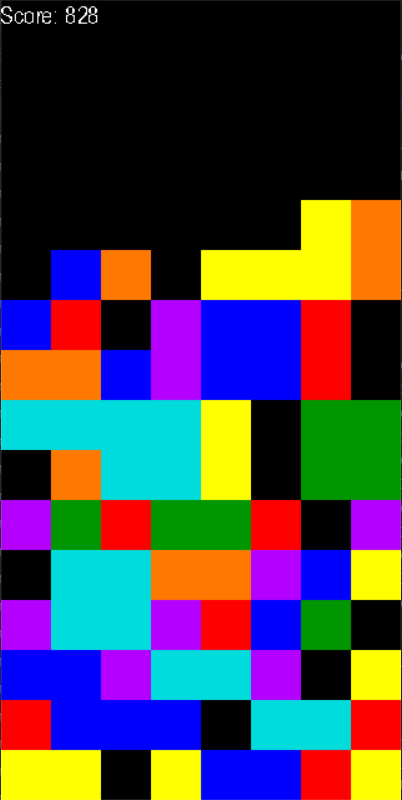
\includegraphics[width=\textwidth]{/tetrisexample2.png}
    	\caption{Example of the game}
    	\label{fig:2}
 	\end{minipage}
\end{figure}

\section{Reinforcement learning}
\subsection{Single neural network}
We started of with the most simplest implantation we could imagine. There is one neural network, which has four input neurons and one output neuron, which must predict the added score of making a move. The input is given four statistics about every move it can play. Before we feed the neural network anything, the game looks at the new block and determines all the possible ways it can end up. It then calculate, for each of these possibilities, the number of holes, the number of full lines (which give points), the total height of the board and the bumpiness of the board (the height difference between two consecutive columns). With these four statistic, the neural network then determines the best score, and this move is then played. The information about this 'round' is then saved to replay memory. When the replay memory contains enough rounds to learn, the neural networks starts to perform Q learning. The target q-value is determined using the Bellman equation. The reward of making a move (the number of lines cleared) is added to the q-value of the state of the board after making the move calculated by the neural network multiplied with a certain discount value. The latter part is in essence the future reward. We usually used a pretty big discount value (0.95) in order to focus much on future reward. We then took this target q-value and used a mean square error loss function with respect to the output of the neural network of the state alone. This can be seen in equation (\ref{eq:loss1}).\\
Additionally we made use of an epsilon greedy strategy. This means we have an exponentially decaying number over the number of episodes which determines how likely the agent is to explore or exploit. Each run a random number is generated. If this random number is higher than the epsilon number, the agent will exploit. If this random number is lower than the epsilon, the agent will explore. \\

\begin{equation}
    \label{eq:loss1}
    \left( Q_{S} - \left(\text{reward} + \text{discount}\cdot Q_{S+1} \right) \right)^2
\end{equation}
In figures (\ref{fig:1NNsimple1}) to (\ref{fig:1NNsimple3}) you can see the average score over 30 episodes for this model for three different learning rates. The other hyperparameters are given in table (\ref{tab:1NN_simple}). We experienced that if the learning rate was too big, as can be seen in figure (\ref{fig:1NNsimple1}), that the loss function became very big and thus the weights also got really big. This phenomenon is called gradient explosion. There are methods to solve this, but we will get to this later. But it can also be solved by using a smaller learning rate. The downside of this is that the system learns very slowly, and may not learn at all once it becomes better, because we then suffer from vanishing gradients. This means that the changes are so small to the weights that they barely make a difference. This can be seen in figure (\ref{fig:1NNsimple2}).
\begin{figure}[h]
	\centering
	\begin{minipage}[b]{0.32\textwidth}
   		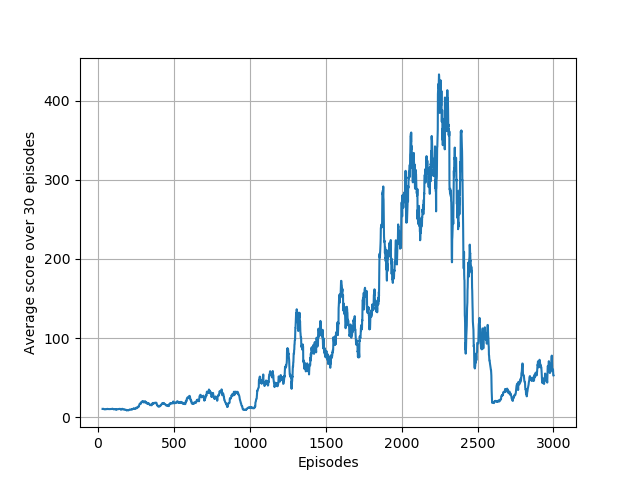
\includegraphics[width=\textwidth]{/ML_1NN_simple_1e-05.png}
    	\caption{learning rate 1e-5}
    	\label{fig:1NNsimple1}
 	\end{minipage}
  	\begin{minipage}[b]{0.32\textwidth}
    	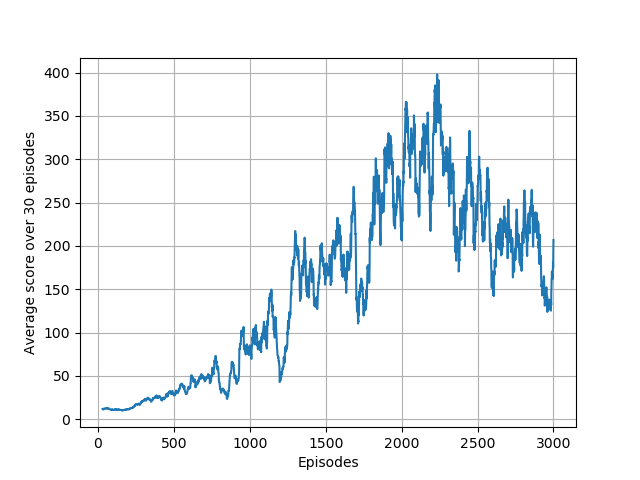
\includegraphics[width=\textwidth]{/ML_1NN_simple_1e-06.png}
    	\caption{learning rate 1e-6}
    	\label{fig:1NNsimple2}
 	\end{minipage}
 	\begin{minipage}[b]{0.32\textwidth}
    	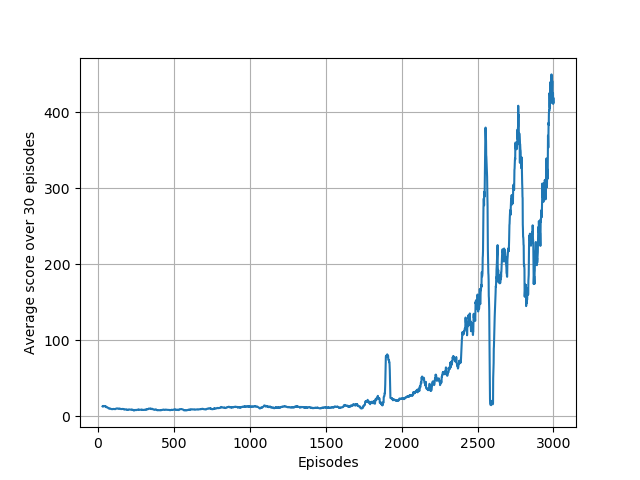
\includegraphics[width=\textwidth]{/ML_1NN_simple_1e-07.png}
    	\caption{learning rate 1e-7}
    	\label{fig:1NNsimple3}
 	\end{minipage}
\end{figure}

\begin{table}[]
    \centering
    \begin{tabular}{|l|l||l|l|}
        \hline
        Parameter & Value & Parameter & Value \\ \hline
        NN hidden layer &  8 neurons with relu & output activation & linear \\
        $\gamma$ & 0.95 & $\epsilon$ decay & 0.002 \\
        batch size & 512 & memory size & 20000 \\
        \hline
    \end{tabular}
    \caption{Hyperparameters for the single NN with stats input}
    \label{tab:1NN_simple}
\end{table}
We also tried using a bigger neural network, where we had two hidden layers consisting of a 16 relu layer and an 8 relu layer. This network was even more sensitive to the hyperparamters and would usually result in very poor results. One successful attempt can be seen in figure (\ref{fig:1NNstate}). It learns at a similar rate to the previous results and does not get much better than around a score of 400. It can be expected that a bigger neural network is more sensitive to the hyperparameters.
\begin{figure}[h]
	\centering
	\begin{minipage}[b]{0.45\textwidth}
   		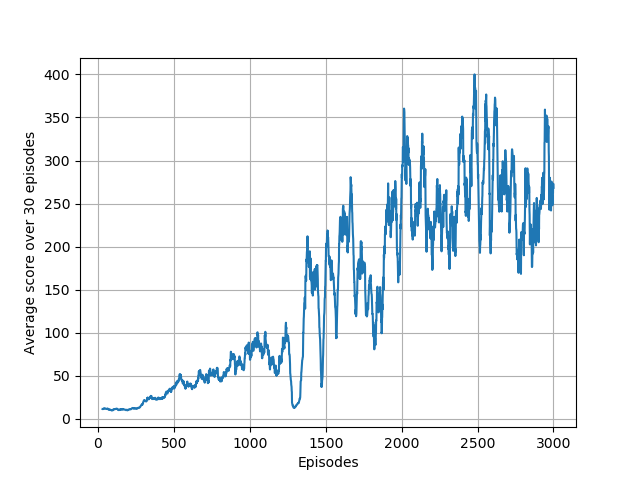
\includegraphics[width=\textwidth]{/ML_1NN_1e-06.png}
    	\caption{learning rate 1e-6}
    	\label{fig:1NNstate}
 	\end{minipage}
  	\begin{minipage}[b]{0.45\textwidth}
    	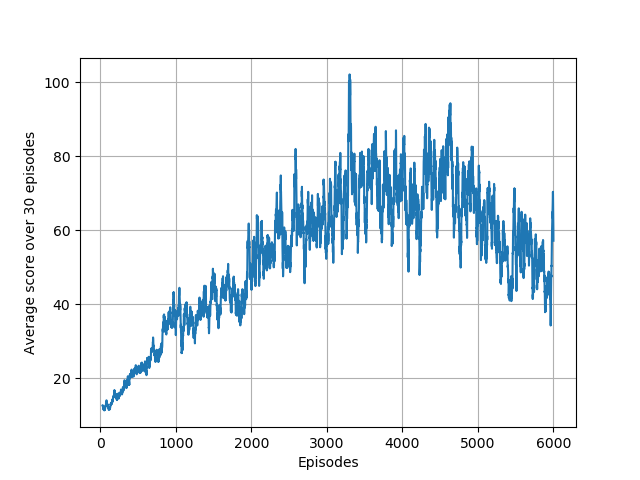
\includegraphics[width=\textwidth]{/ML_1NN_long_1e-05.png}
    	\caption{learning rate 1e-5}
    	\label{fig:1NNboard}
 	\end{minipage}
\end{figure}
Additionally, we also tried another way of feeding the board the the neural network. In this case the input layer of the neural network consisted of $\text{number of columns}\cdot\text{number of rows}$ of the board. In this case we were feeding the entire board for every possible state the block could end up in through the network and determine the score. If a block was present at a certain location, that input would be a one, and if it was empty, the input would be a zero. In this case we used the same hyperparameters as in table (\ref{tab:1NN_simple}), except we used a network consisting out of two hidden layers with 16 relu and 8 relu. The results for a successful learning rate can be seen in figure (\ref{fig:1NNboard}). You can see that the results are pretty poor compared to the state input. We also tried bigger neural networks, but those gave similar results. For this method to work, a bigger network and a more powerful computer are probably required, since more episodes are needed to train such a big network.

\subsection{Comparing our results}
Online we also found some results from people who also tried to use reinforcement learning to play Tetris. Most notable we found a github repository \cite{nlinker}, which gave us the idea to use four statistics about the board as input for the neural network. He used Keras to build his model using Tensorflow as back-end. Keras is a python machine learning package. We also tried using his model, using Keras, on our game and we got results that can be observed in figure (\ref{fig:nlinker}). In this case we used the same hyperparameters as before, except we used a neural network consisting of two hidden layers with both 32 neurons with relu activation. The other main difference was that we used an adam optimiser, which is a more efficient optimiser than SGD, what we used in our own models. You can see that this model does not perform much better than what we have. The author of this model did have very good results in his own project (score $>$ 50000), but he used a bigger board, namely 10x20. When we tried using a bigger board for our own models we saw no significant increase, other than that what can be expected by the fact there simply fit more pieces on the board.
\begin{figure}[h]
	\centering
	\begin{minipage}[b]{0.45\textwidth}
   		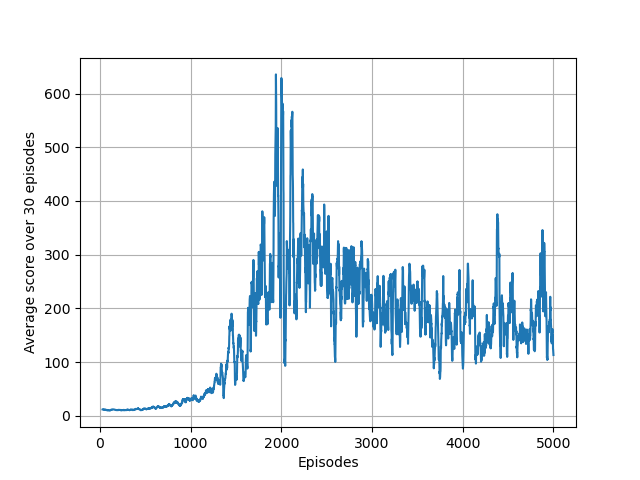
\includegraphics[width=\textwidth]{/nlinker.png}
    	\caption{Results using Keras}
    	\label{fig:nlinker}
 	\end{minipage}
\end{figure}


\subsection{Double neural network}
We also tried a more 'clean' way to handle Q-learning. This means we have two neural networks. The so called policy network and the target network. When all the possible states are calculated by the game, they are fed through the policy network and the best move is played. When the replay memory reaches the point where it contains enough data, the $Q_{S+1}$ in equation (\ref{eq:loss1}) is calculated using the target network and the $Q_S$ is calculated using the policy network. The policy network is then trained using this loss. After a certain number of episodes, the policy network is copied into the target network, so the target network is up to date again. The advantage of the dual network Q-learning over the single network, is that a single network is always kind of chasing its own tail when learning. It needs to calculate $Q_S$ and $Q_{S+1}$ and learn from that, but after it has learning, both those values will have changed for a certain input. It is better (in theory) to have a desperate network determine the $Q_{S+1}$, so that the policy network is not trying to chase its own tail.
We tried this approach for both types of inputs we discussed in the last section.\\
To gather data we ran a lot of simulations for different values of the learning and the target updating rate. We used the same parameters as in table (\ref{tab:1NN_simple}) except that we used a network with two hidden layers, both containing 32 neurons with relu activation. We also tried using the four statistic about the board as input and the whole board as input. Both methods were also very sensitive to the hyperparameters and would usually result in no improvement. There were sometimes multiple combinations of successful hyperparameters and running the same parameters for a second time would sometimes yield a different result. We have shown two of the most successful simulations for the two different input types in figures (\ref{fig:2NNstate}) and (\ref{fig:2NNboard}). You can see that the graph for the statistics input flats out quite quickly after a few hundred episodes. The graph for the board input is still going up, but at such a slow pace that it it would take an eternity to reach a decent level, even assuming that this trend would continue. Based on all the other results maxing out at 100-400, we have no reason to assume this would continue to improve much more. 
\begin{figure}[h]
	\centering
	\begin{minipage}[b]{0.45\textwidth}
   		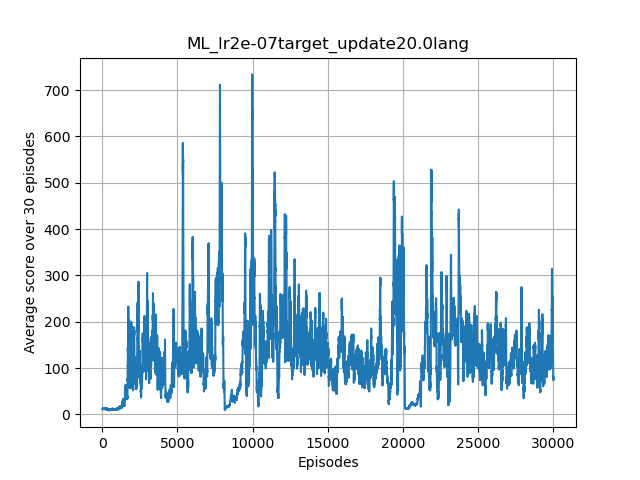
\includegraphics[width=\textwidth]{/2NNstate.png}
    	\caption{learning rate 2e-7 and target update 20 for statistics input}
    	\label{fig:2NNstate}
 	\end{minipage}
  	\begin{minipage}[b]{0.45\textwidth}
    	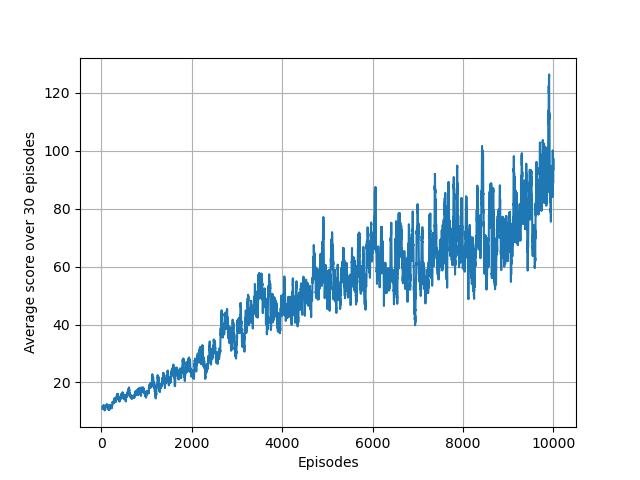
\includegraphics[width=\textwidth]{/2NNboard.png}
    	\caption{learning rate 1e-7 and target update 40 for board input}
    	\label{fig:2NNboard}
 	\end{minipage}
\end{figure}

\section{Neuro-evolution}
We also wanted to try a completely different approach than the reinforcement learning. Another great way to learn a neural network is through an evolutionary algorithm. In this case the members of the population consist of an array containing all the weights and offsets of the entire network. These are then sequentially loaded into the network and tested by playing a game. The members which did the best, and received the highest score, got to live while the other died of and were replaced by combinations of other members. Additionally each gene in a member had a small chance to mutate. We again tried this method for both types of input, the whole board and four statistic about a board. We found that when the input of a whole board was used, the neural network is of course quite large. This meant that the neuro-evolution algorithm was learning, but very slowly as compared to the four statistics input. This method could learn in very big steps.\\
We used a process were the top 25\% of the population went unchanged to the next generation. The 25\% after that was crossed with the member right below them. The 25\% after that was partially crossed with a random member from that same population and the last 25\% consisted of two random members from the population crossed together. But we added in one slight detail. The top performer from the last generation gets copied twice to the next generation. We did this too make sure that if the best member had a bad game due to bad luck, it did not get lost. Before we made this change we sometimes saw a very sudden spike in the score, which died down again after a few generation. After this change, the good member stuck around and improved more rapidly. Besides the crossing, we also had of course a mutation. Every gene of every member had a certain chance to mutate, which was 5\%.\\
We decided to run two long neuro-evolution algorithms for different neural networks. One for a neural network that had as input the four stats about the board, and then two hidden layers with 16 neurons and relu activation for both. The final output layer had a linear activation neuron. For the other we did the same except the second hidden layer consisted out of 8 neurons instead of 16. We did go for the stats input instead of the board input, since the board input would require a lot more weights so the process would take much longer. The results can be found in figures (\ref{fig:evo1}) and (\ref{fig:evo2}). This is the result after letting the training process run for multiple days. You immediately notice the results are way better than the reinforcement learning algorithms, and also much more consistent. Both neural networks give roughly the same results, but the second, figure (\ref{fig:evo2}), seems to have a slight edge over the other with more higher jumps and seemingly a slightly higher average. While the neuro-evolution algorithm definitely seems to be good, it does seem to stop improving quite fast. After about 50 generations both seemed to have stopped improving and were just continuing with the same score.\\
When watching these networks play they almost look like a human playing. They try to make as much full lines as possible and try to minimise the amount of holes. This also seems to be their weakness. They are too determined to not make too much holes, even if it can safe them from dying.\\
A theoretical downside of the neuro-evolution algorithm over the reinforcement algorithm, is that the neuro-evolution algorithm would not learn that is is favourable to clear multiple lines in one turn, since that yields a higher score. It is more focused on staying alive. The reinforcement learning algorithm should in theory be able to learn that clearing multiple lines is good. 
\begin{figure}[h]
	\centering
	\begin{minipage}[b]{0.45\textwidth}
   		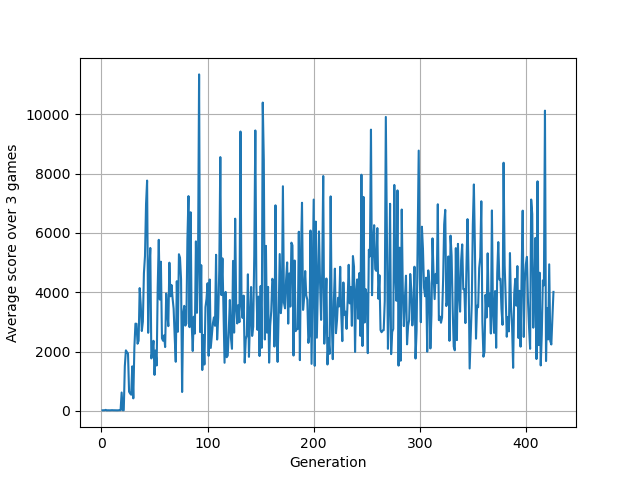
\includegraphics[width=\textwidth]{/evolutionNNstate1616.png}
    	\caption{16 relu 16 relu}
    	\label{fig:evo1}
 	\end{minipage}
  	\begin{minipage}[b]{0.45\textwidth}
    	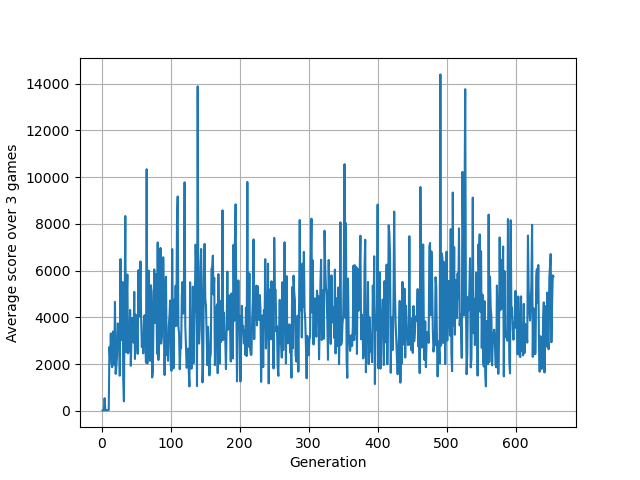
\includegraphics[width=\textwidth]{/evolutionNNstate168.png}
    	\caption{16 relu 8 relu}
    	\label{fig:evo2}
 	\end{minipage}
\end{figure}

\subsection{Conclusion and outlook}
% In the end, we are pretty happy with the results with the neuro-evolution algorithm. It showed that this was for us superior the the reinforcement learning algorithms. But we think there are still improvements to be made here using some more advanced neuro-evolution algorithms, like NEAT. This could be the aim of another project. Additionally, we think the reinforcement learning part of our project can be hugely improved. Another project could focus more on tweaking the hyperparameters, because we saw that very small changes in the hyperparameters could totally destroy the results. Additionally, time could be invested in implementing something that prevents the gradient explosion that we experienced. For example by implementing L2 gradient regularisation. Additionally a better optimiser, like adam, might also make a difference to the results.

In the end, we are pretty happy with the results with the neuro-evolution algorithm. It showed that this was for us superior to the reinforcement learning algorithms. But we think there are still improvements to be made here using some more advanced neuro-evolution algorithms, like NEAT. This could be the aim of another project. For the reinforcement learning part of our project are a lot of improvements possible. For a follow-up project you can think about the following four improvements. First option, focus more on tweaking the hyperparameters, because we saw that very small changes in the hyperparameters could totally destroy the results. Second option, investigating the implementation of something that prevents the gradient explosion that we experienced. For example, by implementing L2 gradient regularisation. Third option, a better optimiser, like Adam, might also make a difference to the results. Fourth, make a combination between reinforcement and evolution like what is done by Gabillon et al. (2013). This will probably very hard to do, but it is the most promising we have seen so far.
All in all, we can be proud on our results. With our approach to the problem we can easily say that the neuro-evolution algorithm works the best, but the reinforcement learning can be improved by a lot, so it is possible that in general reinforcement will be better. This is meanly because it can learn to clear multiple lines at one, what will highly improve your score.


\printbibliography[heading=bibintoc,title={References}]

\end{document}
